\documentclass{article}
\usepackage{amsmath}
\usepackage{tikz}
\usepackage{pgfplots}
\pgfplotsset{compat=1.18}

% Define the viz environment (consumes optional args so they don't render in PDF)
\newenvironment{viz}[1][]{\begin{equation}}{\end{equation}}

\title{LaTeX Visualiser Demo}
\author{Demo}
\date{}

\begin{document}
\maketitle

\section{3D Surfaces}

A paraboloid — hover over the equation in the visualiser to see it in 3D: - works

\begin{viz}[type=surface, label=Paraboloid, xrange=-3:3, yrange=-3:3]
z = x^2 + y^2
\end{viz}

%image
\begin{figure}[h]
  \centering
  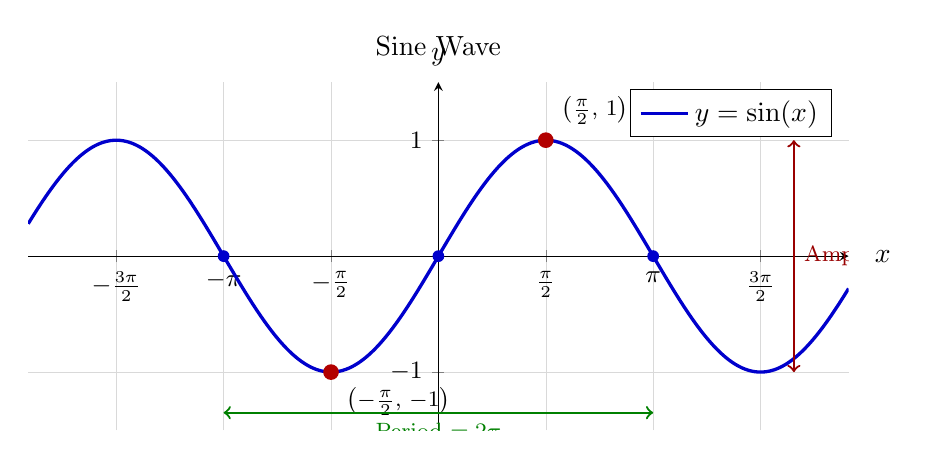
\begin{tikzpicture}
  \begin{axis}[
      width=12cm,
      height=6cm,
      xlabel={$x$},
      ylabel={$y$},
      title={Sine Wave},
      xmin=-6, xmax=6,
      ymin=-1.5, ymax=1.5,
      axis lines=middle,
      grid=major,
      grid style={line width=0.2pt, draw=gray!30},
      samples=200,
      domain=-6:6,
      xtick={-6.28318,-4.7124,-3.14159,-1.5708,0,1.5708,3.14159,4.7124,6.28318},
      xticklabels={$-2\pi$,$-\frac{3\pi}{2}$,$-\pi$,$-\frac{\pi}{2}$,$0$,$\frac{\pi}{2}$,$\pi$,$\frac{3\pi}{2}$,$2\pi$},
      ytick={-1,0,1},
      tick label style={font=\small},
      every axis x label/.style={at={(ticklabel* cs:1.02)}, anchor=west},
      every axis y label/.style={at={(ticklabel* cs:1.02)}, anchor=south},
  ]
  \addplot[
      color=blue!80!black,
      line width=1.2pt,
      smooth,
  ] {sin(deg(x))};
  \addlegendentry{$y = \sin(x)$}
  
  % Annotate key points
  \node[fill=blue!80!black, circle, inner sep=1.5pt] at (axis cs:0,0) {};
  \node[fill=red!70!black, circle, inner sep=2pt, label={[font=\footnotesize]above right:{$\left(\frac{\pi}{2},\,1\right)$}}] at (axis cs:1.5708,1) {};
  \node[fill=red!70!black, circle, inner sep=2pt, label={[font=\footnotesize]below right:{$\left(-\frac{\pi}{2},\,-1\right)$}}] at (axis cs:-1.5708,-1) {};
  \node[fill=blue!80!black, circle, inner sep=1.5pt] at (axis cs:3.14159,0) {};
  \node[fill=blue!80!black, circle, inner sep=1.5pt] at (axis cs:-3.14159,0) {};
  
  % Amplitude annotation
  \draw[<->, thick, red!60!black] (axis cs:5.2,-1) -- node[right, font=\footnotesize]{Amplitude $= 1$} (axis cs:5.2,1);
  
  % Period annotation
  \draw[<->, thick, green!50!black] (axis cs:-3.14159,-1.35) -- node[below, font=\footnotesize]{Period $= 2\pi$} (axis cs:3.14159,-1.35);
  
  \end{axis}
  \end{tikzpicture}
  \caption{TODO: Add caption}
  \label{fig:generated}
\end{figure}


A saddle surface: - doesn't work

\begin{viz}[type=surface, label=Saddle Surface, xrange=-2:2, yrange=-2:2]
z = x^2 - y^2
\end{viz}

\section{2D Curves}

The classic sine wave:

\begin{viz}[type=curve, label=Sine Wave, xrange=-6:6]
y = \sin(x)
\end{viz}



A polynomial:

\begin{viz}[type=curve, label=Cubic, xrange=-3:3]
y = x^3 - 3x
\end{viz}

\section{More Complex Surfaces}



A ripple function:

\begin{viz}[type=surface, label=Ripple, xrange=-4:4, yrange=-4:4]
z = \sin(x^2 + y^2)
\end{viz}

A Gaussian bump:

\begin{viz}[type=surface, label=Gaussian, xrange=-3:3, yrange=-3:3, colorscale=Plasma]
z = \exp(-(x^2 + y^2))
\end{viz}





\end{document}